\begin{frame}[c]
    \frametitle{基于线性可变滤光片的亚纳米分辨率显微光谱仪的设计与实现}
    \begin{itemize}
        \item Emadi, A.;  Wu, H.;  de Graaf, G.; Wolffenbuttel, R., Design and implementation of a \textcolor{purple}{sub-nm resolution} microspectrometer based on a  \textcolor{red}{Linear-Variable Optical Filter}. Optics Express 2012, 20 (1), 489-507.
        \item \textcolor{blue}{创新点:}光谱分辨率基本上取决于探测器的数量。
        \item \textcolor{blue}{瓶颈:}一般用于相对狭窄的光谱波段:$610\sim 680\ \mathrm{nm}$(分辨率 0.7 nm)、$570\sim 740\ \mathrm{nm}$(分辨率 2.2 nm)。
    \end{itemize}
    仪器结构示意图:(相当于一系列连续变化的法布里-珀罗(FP)谐振腔)
    \begin{figure}[H] %H为当前位置,!htb为忽略美学标准,htbp为浮动图形
        \centering %图片居中
        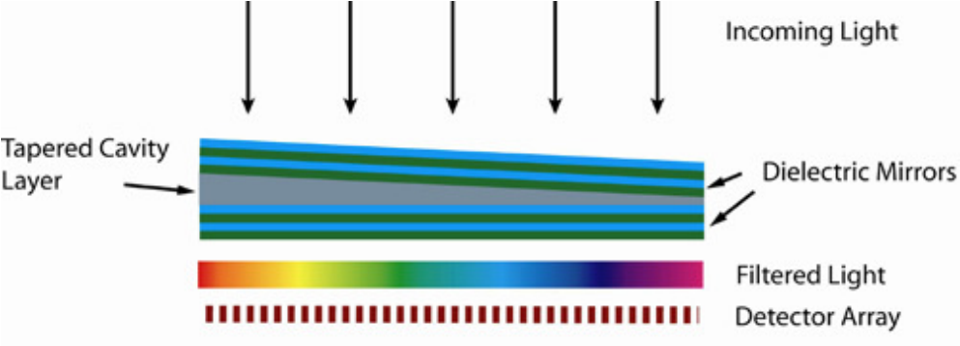
\includegraphics[width=1.\textwidth]{figures/Design and implementation of a sub-nm resolution microspectrometer based on a Linear-Variable Optical Filter_1.png} %插入图片,[]中设置图片大小,{}中是图片文件名
    \end{figure}
\end{frame}

\begin{frame}[c]
    \frametitle{基于线性可变滤光片的亚纳米分辨率显微光谱仪的设计与实现}
    薄膜结构:$\downarrow$ light
    \begin{itemize}
        \item $\mathrm{TiO}_2(68.5\ \text{nm})-\mathrm{SiO}_2(112\ \text{nm})-\mathrm{TiO}_2-\mathrm{SiO}_2-\mathrm{TiO}_2-\mathrm{SiO}_2-\mathrm{TiO}_2$
        \item $\mathrm{SiO}_2(800 \sim 1050 \text{nm})$
        \item $\mathrm{TiO}_2(68.5\ \text{nm})-\mathrm{SiO}_2(112\ \text{nm})-\mathrm{TiO}_2-\mathrm{SiO}_2-\mathrm{TiO}_2-\mathrm{SiO}_2-\mathrm{TiO}_2$
        \item Substrate: Glass
    \end{itemize}
    \begin{columns}
        \begin{column}{.5\textwidth}
            滤光效果:
            \begin{figure}[H] %H为当前位置,!htb为忽略美学标准,htbp为浮动图形
                \centering %图片居中
                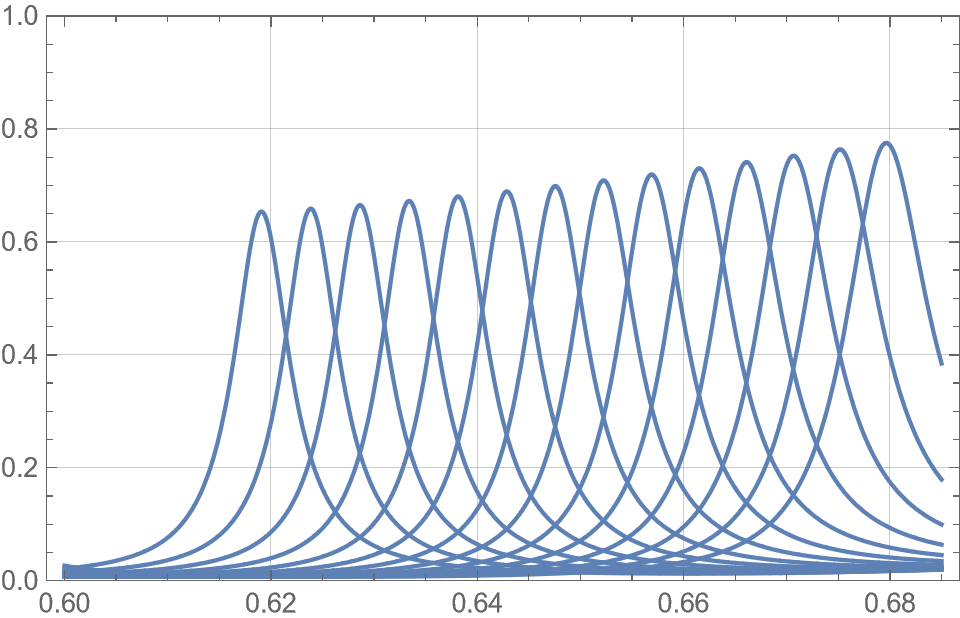
\includegraphics[width=1.\textwidth]{figures/Design and implementation of a sub-nm resolution microspectrometer based on a Linear-Variable Optical Filter_3.png} %插入图片,[]中设置图片大小,{}中是图片文件名
            \end{figure}
            沉积工艺见右(从上到下)$\rightarrow\rightarrow\rightarrow$

            文章后面还给出了数据处理的算法以及实验结果、和其他仪器的比较
        \end{column}
        \begin{column}{.5\textwidth}
            \begin{figure}[H] %H为当前位置,!htb为忽略美学标准,htbp为浮动图形
                \centering %图片居中
                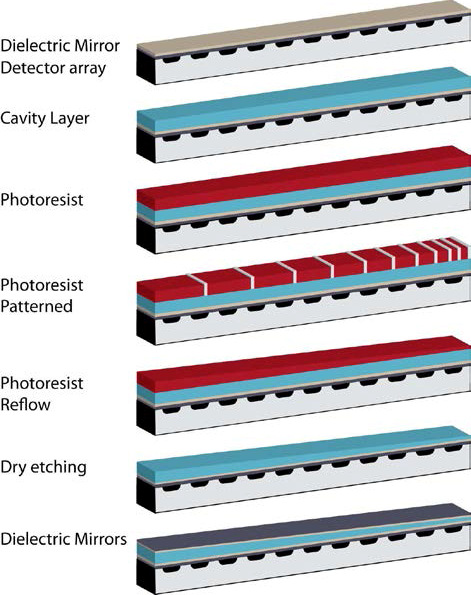
\includegraphics[width=1.\textwidth]{figures/Design and implementation of a sub-nm resolution microspectrometer based on a Linear-Variable Optical Filter_2.png} %插入图片,[]中设置图片大小,{}中是图片文件名
            \end{figure}
        \end{column}
    \end{columns}
\end{frame}